\documentclass[a4paper, 12pt]{article}

\usepackage{amsmath}
\usepackage{array}
\usepackage{hyperref}
\usepackage{cleveref}
\hypersetup{
	colorlinks=true,
	linkcolor=blue,
	filecolor=blue,
	citecolor = black,
	urlcolor=cyan,
}

\usepackage{graphicx}
\usepackage{caption}
\usepackage[section]{placeins}
\usepackage{lipsum}


%for code(MATLAB in particular)
\usepackage{listings}
\usepackage{color} %red, green, blue, yellow, cyan, magenta, black, white
\definecolor{mygreen}{RGB}{28,172,0} % color values Red, Green, Blue
\definecolor{mylilas}{RGB}{170,55,241}

\lstset{
    language=Matlab,%
    %basicstyle=\color{red},
    breaklines=true,%
    morekeywords={matlab2tikz},
    keywordstyle=\color{blue},%
    morekeywords=[2]{1}, 
    keywordstyle=[2]{\color{black}},
    identifierstyle=\color{black},%
    stringstyle=\color{mylilas},
    commentstyle=\color{mygreen},%
    showstringspaces=false,%without this there will be a symbol in the places where there is a space
    numbers=left,%
    numberstyle={\tiny \color{black}},% size of the numbers
    numbersep=7pt, % this defines how far the numbers are from the text
    emph=[1]{for,end,break},
    emphstyle=[1]\color{red}, %some words to emphasise
    %emph=[2]{word1,word2}, emphstyle=[2]{style},
}


\graphicspath{{./pictures/}}

\title{ECEN315 - Assignment 2}
\author{Joshua Benfell - 300433229}

\begin{document}
    \maketitle

    \section{Question 1}
        \lstinputlisting{../q1.m}
        
        \begin{table}[!h]
            \caption{Time Constants and Settling Time for Various Step Inputs}
            \label{tab:q1}
            \centering
            \begin{tabular}{r|c|r}
                Step Size & Time Constants & Settling Time\\
                \hline
                1 & $\begin{pmatrix} 3.7321 \\ 0.2679 \end{pmatrix}$ & 14.879\\
                2 & $\begin{pmatrix} 1.7071 \\ 0.2929 \end{pmatrix}$ & 6.9996\\
                4 & $\begin{pmatrix} 5 \\ 5 \end{pmatrix}$ & 2.1970\\
                8 & $\begin{pmatrix} 5 \\ 5 \end{pmatrix}$ & 2.1082

            \end{tabular}
        \end{table}

        \begin{figure}[!h]
            \centering
            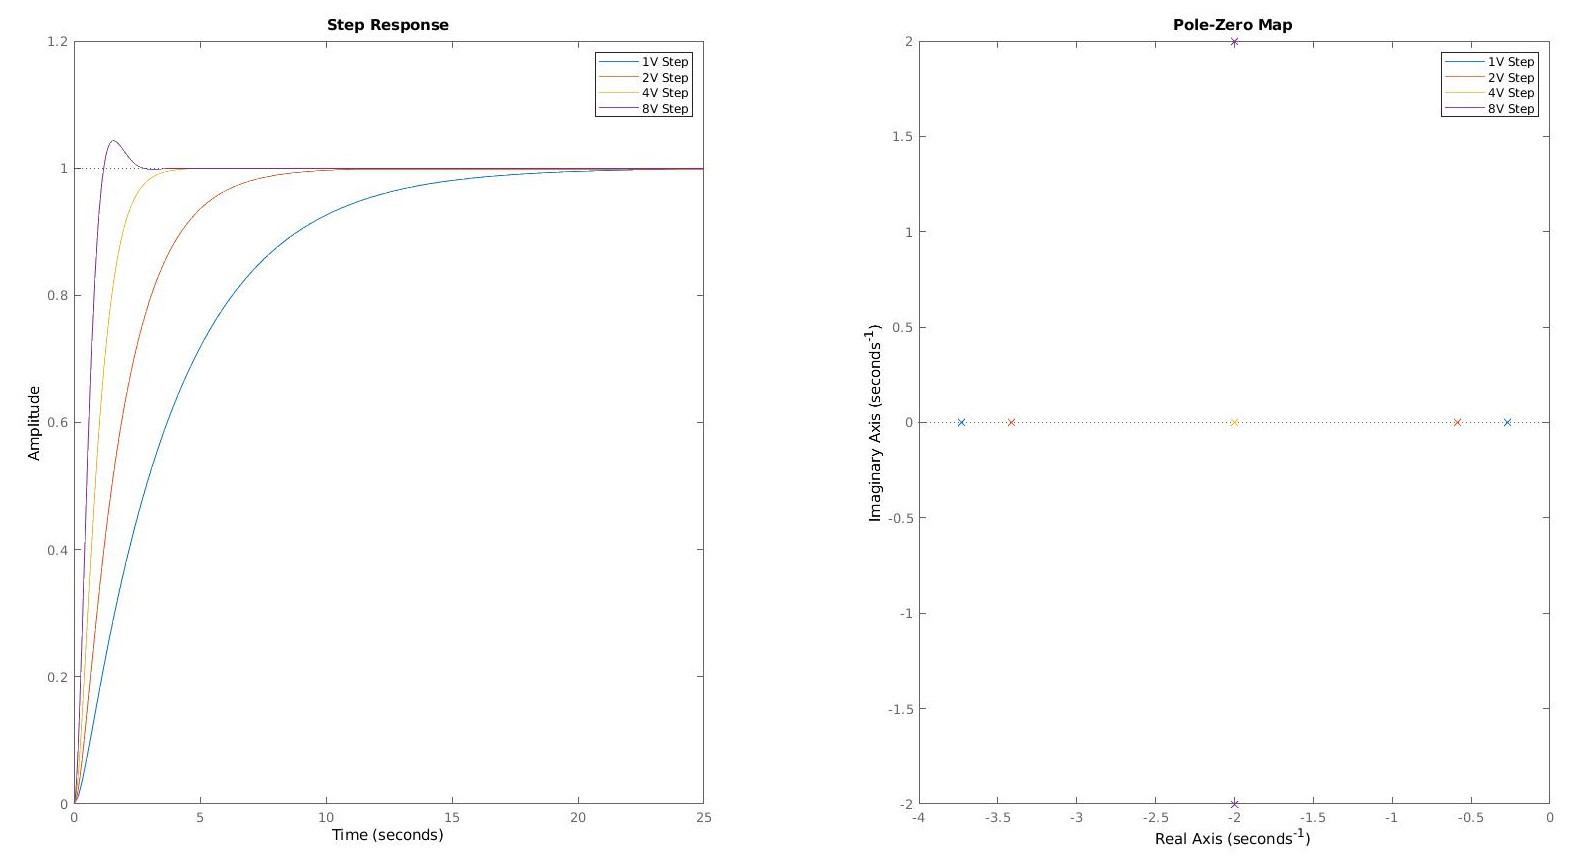
\includegraphics[width=\textwidth]{q1.jpg}
            \caption{Step Response to various step sizes and PZ Map of those step responses}
            \label{fig:q1}
        \end{figure}

    \section{Question 2}

        \lstinputlisting{../q2.m}

        \begin{figure}[!h]
            \centering
            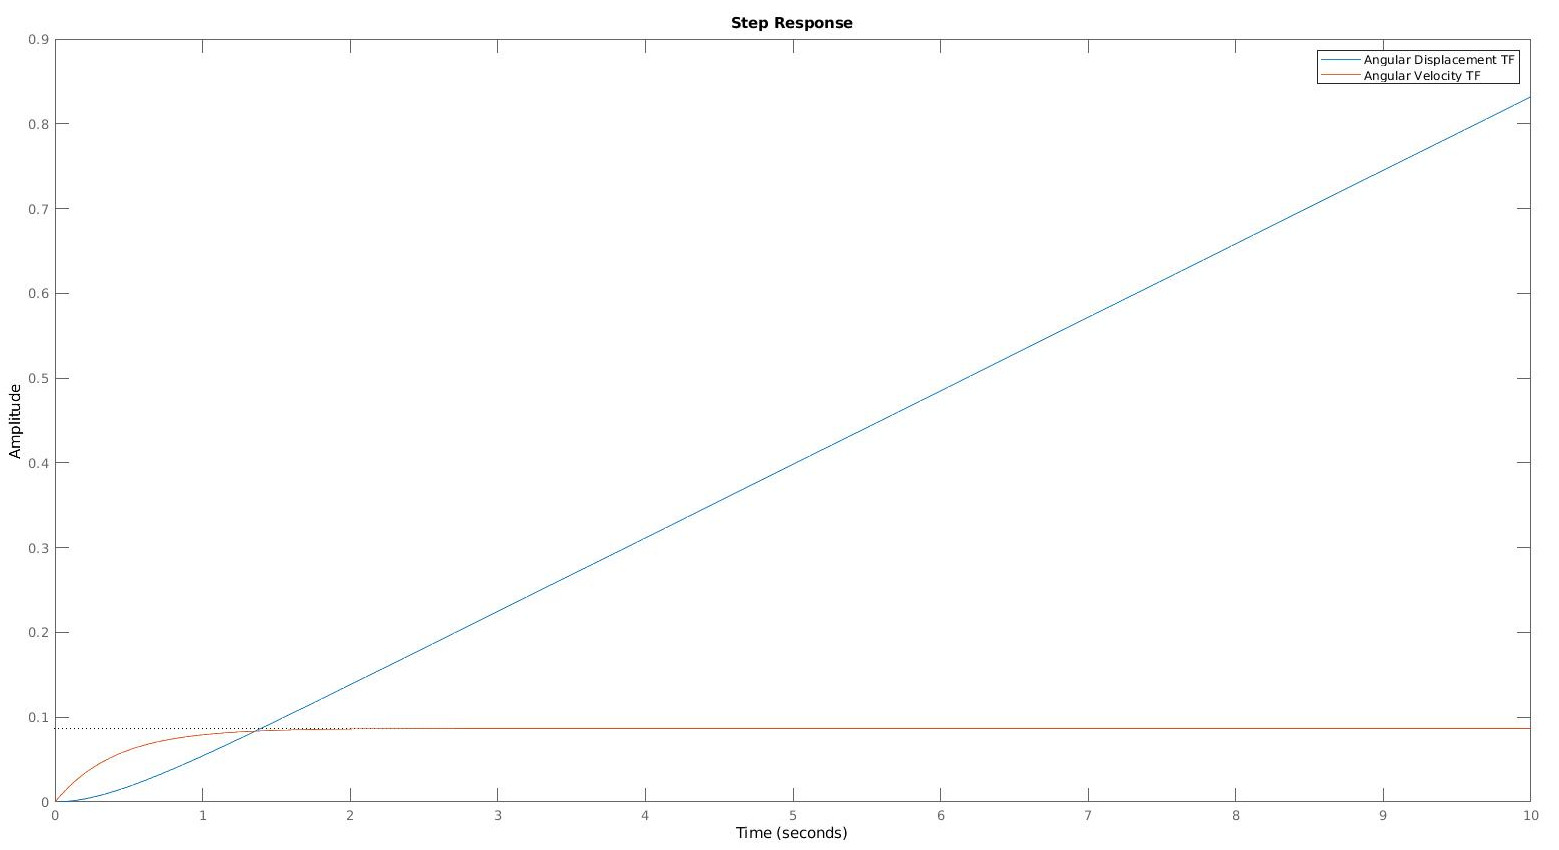
\includegraphics[width=\textwidth]{q2.jpg}
            \caption{Step Response of $\frac{\Theta_L(s)}{E_a(s)}$ and $\frac{\Omega_L(s)}{E_a(s)}$}
            \label{fig:q2}
        \end{figure}

    \section{Question 3}

        \lstinputlisting{../q3.m}
        \begin{table}[!h]
            \centering
            \caption{Relevant values for the systems defined in question 3}
            \label{tab:q3}
            \begin{tabular}{l|r|r|r|r|r|r}
                System & $\omega_n$ & $\zeta$ & $T_s$ (s) & $T_p$ (s) & $T_R$ (s) & $OS\%$ \\ 
                \hline
                $G_1(s)$ & $4$   & $0.375$ & $2.66$ & $0.86$ & $0.357$ & $28$ \\
                $G_2(s)$ & $0.2$ & $0.05$  & $3.8$  & $15.7$ & $5.42$  & $85.4$ \\
                $G_3(s)$ & $3.2711 \times 10^3$ & $0.2446$ & $0.00433$ & $0.000979$ & $0.0003864$ & $45.2$
                
            \end{tabular}
        \end{table}

        \begin{figure}[!h]
            \centering
            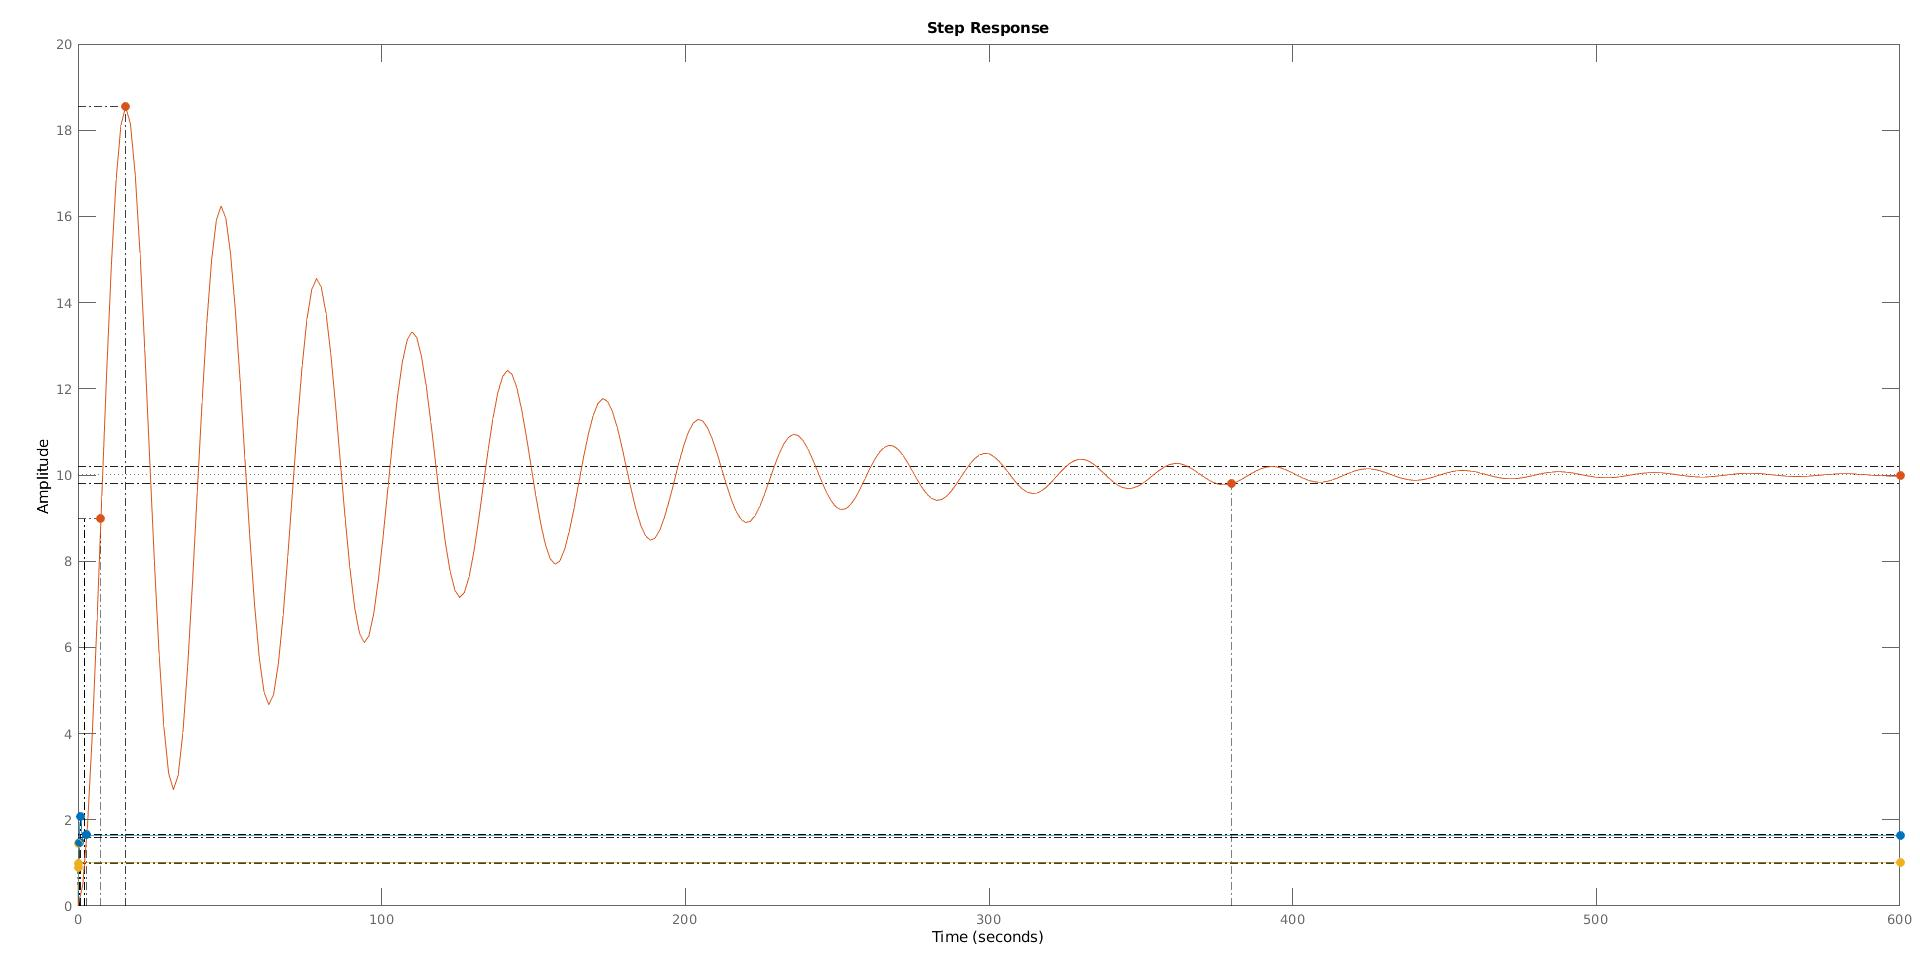
\includegraphics[width=\textwidth]{q3.jpg}
            \caption{Usage of the LTI Viewer exported to figure}
            \label{fig:q3}
        \end{figure}

    \section{Question 4}

        \lstinputlisting{../q4.m}

        \begin{figure}[!h]
            \centering
            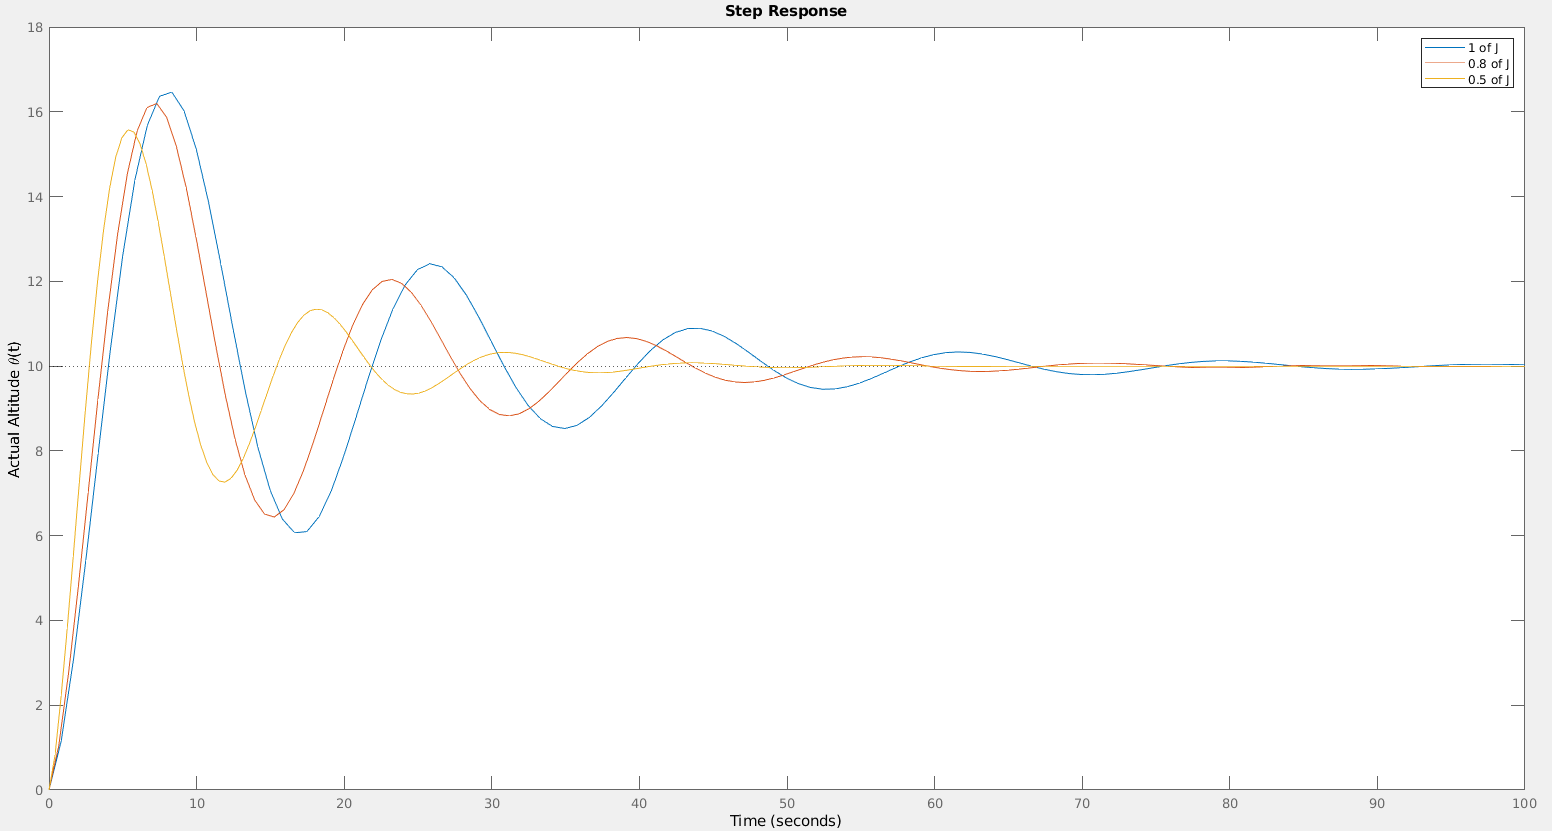
\includegraphics[width=\textwidth]{q4.png}
            \caption{Satellite Step Responses for various moments of inertia}
            \label{fig:q4}
        \end{figure}

    \section{Question 5 (6 in the handout)}

        \lstinputlisting{../q6.m}

        \begin{figure}[!h]
            \centering
            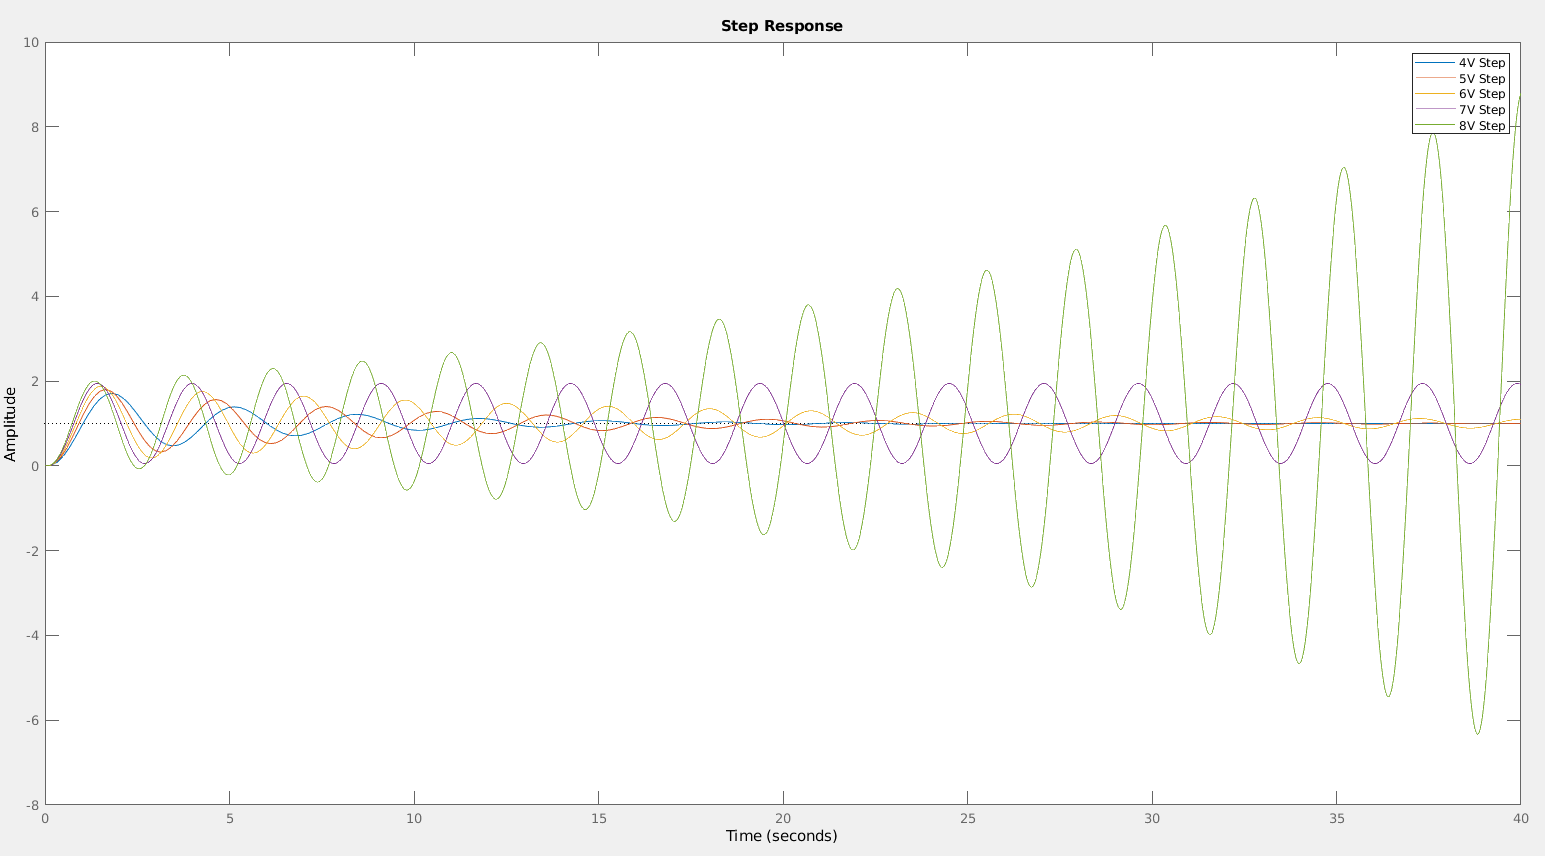
\includegraphics[width=\textwidth]{q5.png}
            \caption{Gain Controller Step Response Stability}
            \label{fig:q5a}
        \end{figure}

        \begin{figure}[!h]
            \centering
            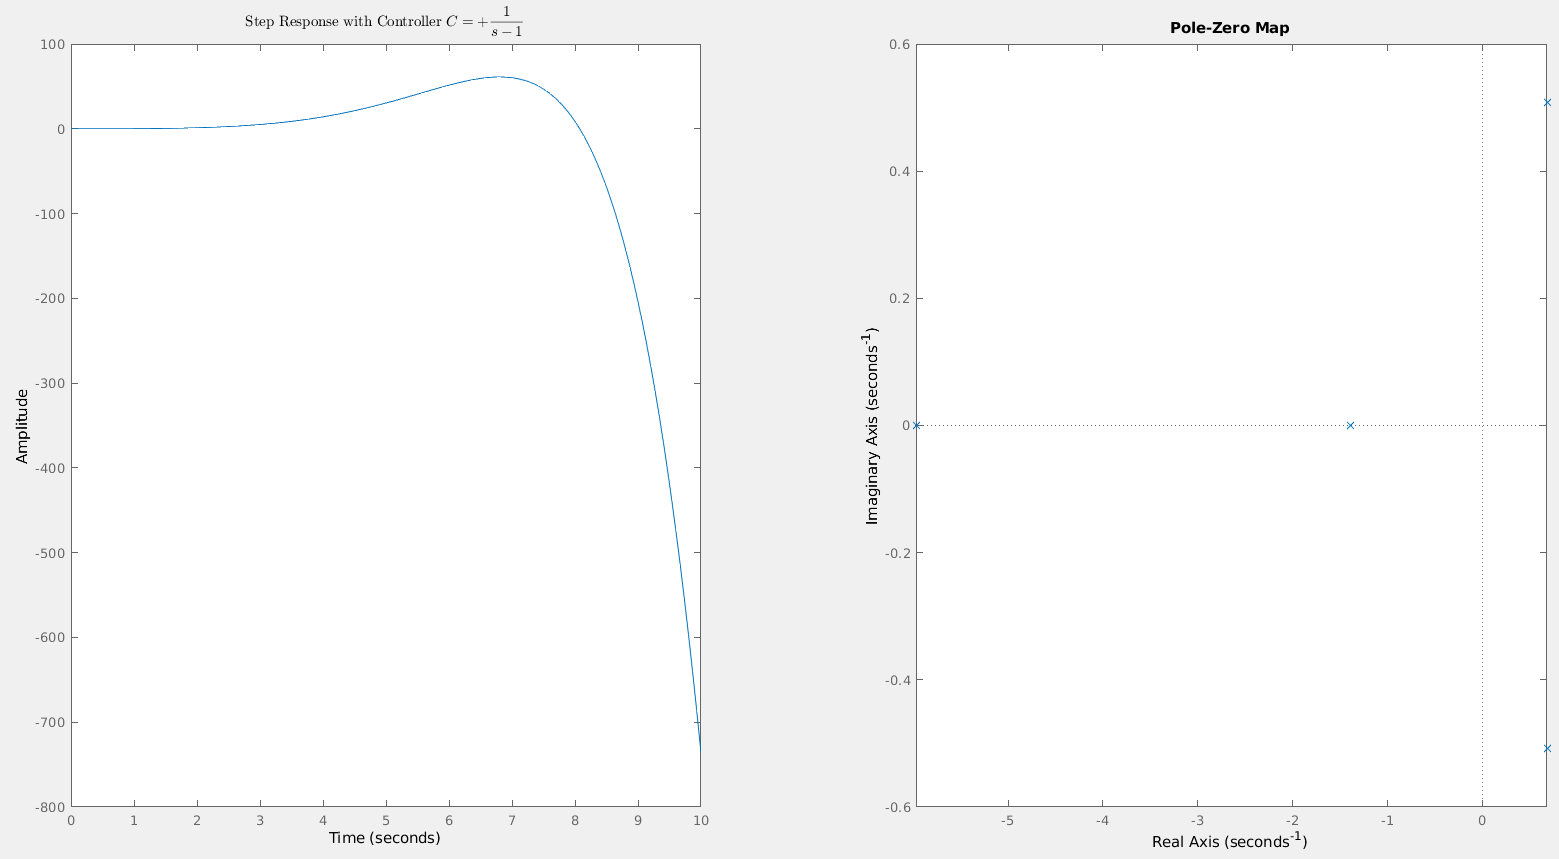
\includegraphics[width=\textwidth]{q5b.png}
            \caption{PI Controller Stability with low steady state gain}
            \label{fig:q5b}
        \end{figure}

\end{document}